\documentclass[12pt]{article}
\usepackage{graphicx}
%\usepackage{subcaption}
\usepackage{caption}
\usepackage{mathtools}
\usepackage{tikz,pgfplots}
\usepackage{subfig}
\usepackage{epsfig}
\usepackage{amsmath}
\usepackage{amssymb}
\usepackage[shortlabels]{enumitem}
\usetikzlibrary{angles,patterns,calc}
\usepackage{bbm}
\usepackage{float}
\newcommand\der[2]{\frac{\partial{#1}}{\partial{#2}}}
\DeclareMathOperator*{\argmax}{arg\,max}
\DeclareMathOperator*{\argmin}{arg\,min}

% stuff to put matlab code in 
\usepackage{listings}
\usepackage{color} %red, green, blue, yellow, cyan, magenta, black, white
\definecolor{mygreen}{RGB}{28,172,0} % color values Red, Green, Blue
\definecolor{mylilas}{RGB}{170,55,241}

% Shortcut greek
\def\a{\alpha}
\def\b{\beta}
\def\g{\gamma}
\def\D{\Delta}
\def\d{\delta}
\def\z{\zeta}
\def\k{\kappa}
\def\l{\lambda}
\def\n{\nu}
\def\r{\rho}
\def\s{\sigma}
\def\t{\tau}
\def\x{\xi}
\def\w{\omega}
\def\W{\Omega}

\usepackage[utf8]{inputenc}
\usepackage[english]{babel}
\usepackage{fancyhdr}
\fancypagestyle{firststyle}
{
\fancyhf{}
    \renewcommand{\headrulewidth}{0pt}
   \fancyfoot[C]{\footnotesize Page \thepage\ of \pageref{LastPage}}
}

\newcommand{\numpy}{{\tt numpy}}    % tt font for numpy

\topmargin -.5in
\textheight 9in
\oddsidemargin -.25in
\evensidemargin -.25in
\textwidth 7in

\newcommand{\question}[1]{ \begin{center} \noindent\colorbox{gray!10}{
\parbox{0.8\textwidth}{\vspace{0.125in} #1 \vspace{0.125in} } } \end{center} }

\begin{document}

    \thispagestyle{firststyle}

    \author{Isaac Liu, Nicol\'as Martorell \& Paul Opheim}
    \title{Attenuation Bias, Measurement Error \& Principal Component Analysis} 
    \maketitle

    % code

    \lstset{language=Matlab,%
        %basicstyle=\color{red},
        breaklines=true,%
        morekeywords={matlab2tikz},
        keywordstyle=\color{blue},%
        morekeywords=[2]{1}, keywordstyle=[2]{\color{black}},
        identifierstyle=\color{black},%
        stringstyle=\color{mylilas},
        commentstyle=\color{mygreen},%
        showstringspaces=false,%without this there will be a symbol in the places where there is a space
        numbers=left,%
        numberstyle={\tiny \color{black}},% size of the numbers
        numbersep=9pt, % this defines how far the numbers are from the text
        emph=[1]{for,end,break},emphstyle=[1]\color{red}, %some words to emphasise
        %emph=[2]{word1,word2}, emphstyle=[2]{style},    
    }

    \begin{abstract}

        Shorter version of the abstract (I would say 4-5 sentences in a single paragraph max) goes here
        
    \end{abstract}

    \newpage \clearpage

    % Introduction (no need for a section header for this)

        Many variables of interest in economics are not directly available as empirical data. Instead, economists often use other variables that are imperfect measurements of the true focus of their analysis. These available variables are known as \textit{proxies} or ``variables measured with error'', and, if they suffer from classical measurement error, their use causes \textit{attenuation bias} when they are used as independent variables in econometric estimation. Traditionally, instrumental variables are used as a shock of exogeneity to get rid of this bias, but finding truly exogenous variables that satisfy the exclusion restriction is difficult, and so this method can often not be feasibly applied.

        As an alternative to dealing with attenuation bias, we propose the use of Principal Component Analysis (PCA) over several variables measured with error. When there are multiple observed variables driven by a single ``true'' one, we propose to use PCA over these variables to extract the ``true'' variable. We then use this extracted value and use it in a standard OLS regression, thus providing a solution to attenuation bias that does not require the strong assumptions of instrumental variable analysis.

        To show the properties and behaviour of our estimator on large samples under standard assumptions, we present a theoretical framework and a Monte-Carlo analysis. Additionally, we explore a basic empirical application to our method, by estimating the effect of economic development on life expectancy at birth. Since there is no consensus on how to measure economic development, we take a sample of different variables that may measure economic development with error (GDP per capita, GNI per capita, Household Income Per Capita, among others) over which we apply PCA to apply our identification strategy.

    \section*{Literature}

        Brief discussion of https://warwick.ac.uk/fac/soc/economics/staff/knagasawa/PartialEffects.pdf, as well as anything else important that comes up on Google Scholar

        So it actually kind of seems like we are doing something unique, but it's not clear that what we are doing is better than existing approaches to measurement error. Like averaging or instrumenting variables with each other.

        Nagasawa 2020 
        theoretically develops the use of a proxy variable to deal with unobserved heterogeneity in line with the definitions in the measurement error literature
        Uses an imperfect measurment of the error, the proxy
        problem is in nuisance parameters
        has a single proxy variable
        nonparametric approach mentioned as having limited usefulness due to curse of dimensionality and restrictive common support
        kernel first stage
        new partial effects method of proxy

        % https://www-annualreviews-org.proxy.uchicago.edu/doi/pdf/10.1146%2Fannurev-economics-080315-015058
        Schennach 2016
        focuses on nonclassical measurement error and nonlinear cases- classical cases 'uninteresting' because IV is very easy to use
        relaxing common assumptions
        origins and simple approaches
        validation data or repeated measurements
        proxies are related to the variable of interest but maybe nonlinearly... indicators may be instruments
        time series and panel repetition
        factor high and low dimensional relations
        multivariate linear regresison- worse than attenuation bias... and nonlinear models lead IV to fail.
        repeated measurments- old lemma. nonparametric density estimation
        moments apporach and polynomials, basis and transforms, etc.
        symmetric kernel smoothing
        factor models- x is informed by factor loadings plus noise- latent
        covariance identification. normalization is needed.
        SEE HECKMAN 2010A
        control variables- NO need for normalization
        with the matrix known construct vectors of repeated measurment and decompose
        nonlinear exxtension.
        iv more general and can be biased... polynomial paramteric
        identificaiton is difficult in this nonlinear situation
        quantile regression possilbity
        panel data- future values can give information.

        %https://advstats.psychstat.org/book/factor/index.php#factor-analysis
        factor analysis can handle measurement errors in multiple ways
        exploratory factor analysis can be used to explore dimensionality of measurement instrument (like prof mentioned i guess). I think this is like just the PCA step and looking at the Loadings
        confirmatory factor analysis-test if constructs influence responses
        some unique observation factors
        there is discussion of the variance of the true variable and the variance of the measurmenet error.
        i think there might be misuse of the term measurement errors/this is not clear
        overall not very related

        %http://web.pdx.edu/~newsomj/semclass/ho_latent.pdf
        latent variable models... are really basically mathematically the same as measurement error
        simple and standard me explanation
        reminder- standardized coefificetn is very similar to correlation coefficient
        reminder that there is no impact of measurmeent error in y on unstandardized coeff
        multiple regression- x1 coeff can indeed be biased, middle of p.2
        lower statistical power
        no bias in the mean of x
        bad impact on the regression
        use Structural Equation Modelling to estimate path coefficients among latent variables
        need three or more measures to estimate a latent variable
        in a footnote it mentions a case with only two indicators
        not always me but sometimes uniqueness... really it's just items unaccounted for by the factor
        latent variance is independent.. classical assumption

        Wegge
        %https://www.sciencedirect.com/science/article/pii/0304407694016763
        measurment error regression models are factor analysis mdoels, with the correct regressors being the factors. indeed. but no common stat method, because true factors not known- no clear coeffiicent linkage. instead, grouping
        dependent variables and latent factors uncorrelated with errors
        counting rules
        data grouping remedies- structural equations
        grouped regression model- ivs and weighted averages of ivs
        if there is very little credible info about the variance of measurment errors or the covariance of equation erros, factor loading restrictions are needed for identification
        this paper is about identification and IVs really

        %https://www.ncbi.nlm.nih.gov/pmc/articles/PMC4787301/
        schoefield
        mixed effects structural equations model
        combine structural equations and item response theory
        attenuation, or nonclassical bias in any direction
        clear misestimation consequences
        solutions in IV or nonparametric bounds. here IRT
        error structure assumed by IV often violated
        bayesian structural framework and model
        this paper is focused on ME in the main regressor

        %http://jenni.uchicago.edu/econ374/papers/Heckman_Schennach_Williams_2011_lin_lin_matching_2011-10-03a_cji.pdf
        heckman 2010
        the abstract makes it very clear that this is a paper in a similar situation, except involving matching
        it is incomplete, however
        matching estimators can be harmed by mismeasured conditioning variables
        however, average treatment effects can be identified using factor models with quality proxies
        there often is not a need for normalization

        *perhaps note somewhere that governmnet spending is less likely to have measurement error because it's an official statistic... though health spending in the denominator could have error... ow.

    \section*{Theoretical framework}

        Consider a model where the outcome is denoted by $y_i$. This outcome depends on a variable of interest denoted by $t_i$ and a vector of covariates denoted by $X_i=(x_{i,1},x_{i,2},\dots x_{i,p})'$. Additionally, consider a vector of variables $X^*_i=(x^*_{i,1},x^*_{i,2},\dots x^*_{i,p})'$ that correspond to the covariates $X_i$ but observed with measurement error, where $x^*_{i,k}=x_{i,k}+\eta_{i,k}$ with $\eta_{i,k} \sim {iid}(0,\sigma^2_{\eta_k})$, $\operatorname{E}(x_{i,k}'\eta_{i,k})=0, \forall i$, $\operatorname{E}(x_{i,k}'\eta_{j,l})=0, \forall i\neq j$ and $k \neq l$, and $\operatorname{E}(\eta_{i,k}'\eta_{j,l})=0, \forall i\neq j$ and $k \neq l$. Therefore, each $x^*_{i,k}$ suffers from classical measurement error. Note that $\operatorname{E}(x_{i,k})=\operatorname{E}(x^*_{i,k})=\mu_{x_k}$ and that $\operatorname{V}(x_{i,k})=\sigma^2_{x_k}$ while $\operatorname{V}(x^*_{i,k})=\sigma^2_{x_k}+\sigma^2_{\eta_k}\geq \sigma^2_{x_k}$.

    \subsection*{Data Generating Process}

        Assume that the outcome $y_i$ is determined by the following Data Generation Process (DGP):
        \begin{align}
            y_i = \gamma t_i + X_i'\beta + \epsilon_i
        \end{align}

        where $\g$ is the parameter of the variable of interest $t_i$, $\b=(\b_1,\b_2,\dots \b_p)'$ is the vector of the parameters of the covariates $X_i$ including a constant and $\epsilon_i \sim \operatorname{iid}(0,\sigma^2_\epsilon)$. Under this specification, the coefficients are such that:
        \begin{align}
            \left(\begin{array}{l}
        {\gamma} \\
        {\beta}
        \end{array}\right)=\left(\begin{array}{cc}
        {\sigma}^2_{t} & \Sigma_{tX} \\
        \Sigma_{Xt} & {\Sigma}_{X}
        \end{array}\right)^{-1}\left(\begin{array}{c}
        \Sigma_{yt} \\
        \Sigma_{yX}
        \end{array}\right)
        \end{align}

        Suppose that the econometrician has access to $t_i$ but, instead of $X_i$ she observes $X^*_i$. Then, she specifies the following linear model
        \begin{align}
            y_i = \gamma^* t_i + {X^{*}_i}' \beta^* + \zeta_i
        \end{align}

        the coefficients would be such that
        \begin{align}
            \left(\begin{array}{l}
        {\gamma}^* \\
        {\beta}^*
        \end{array}\right)&=\left(\begin{array}{cc}
        {\sigma}^2_{t} & \Sigma_{tX^*} \\
        \Sigma_{X^*t} & {\Sigma}_{X^*}
        \end{array}\right)^{-1}\left(\begin{array}{c}
        \Sigma_{yt} \\
        \Sigma_{yX^*}
        \end{array}\right) \\
        & =\left(\begin{array}{cc}
        {\sigma}^2_{t} & \Sigma_{tX} \\
        \Sigma_{Xt} & {\Sigma}_{X}+{\Sigma}_{\eta}
        \end{array}\right)^{-1}\left(\begin{array}{cc}
        {\sigma}^2_{t} & \Sigma_{tX} \\
        \Sigma_{Xt} & {\Sigma}_{X}
        \end{array}\right)\left(\begin{array}{l}
        {\gamma} \\
        {\beta}
        \end{array}\right)
        \end{align}

        To the see the implications of the of this measurement error in the covariates, consider a simple case where the DGP depends only of the variable of interest and a covariate such that:

        \begin{align}
            \left(\begin{array}{l}
        {\gamma} \\
        {\beta}
        \end{array}\right)=\left(\begin{array}{l}
        1 \\
        1
        \end{array}\right)
        \end{align}

        and with $\sigma^2_t=\Sigma_X=\Sigma_\eta=1$ while $\Sigma_{Xt}=0.6$. Then
        \begin{align*}
            \left(\begin{array}{l}
        {\gamma}^* \\
        {\beta}^*
        \end{array}\right)& =\left(\begin{array}{cc}
        1 & 0.6 \\
        0.6 & 2
        \end{array}\right)^{-1}\left(\begin{array}{cc}
        1 & 0.6 \\
        0.6 & 1
        \end{array}\right)\left(\begin{array}{l}
        1\\
        1
        \end{array}\right) \\
        \left(\begin{array}{l}
        {\gamma}^* \\
        {\beta}^*
        \end{array}\right)&=\left(\begin{array}{l}
        1.37 \\
        0.39
        \end{array}\right)
        \end{align*}

        Clearly, both coefficients shows bias when the econometrician assumes a DGP with $X_i^*$: while there is attenuation bias on the coefficient of the covariate, the coefficient of the variable of interest is biased upward given that some of the effect of the covariates is ``omitted'' given this attenuation.

    \subsection*{Instrumental Variables Regression as a Bias-Correction Method}

        The classical solution for the measurement-error induced bias in econometrics has been the usage of instrumental variables. Suppose an instrument $Z_i$ that satisfies the relevance condition $\operatorname{E}(Z_i'X_i)\neq 0$ and $\operatorname{E}(Z_i't_i)\neq 0$, and also the exclusion restriction $\operatorname{E}(Z_i'\epsilon_i)=\operatorname{E}(Z_i'\zeta_i)=\operatorname{E}(Z_i'\eta_{i,k})=0$, for all $i$ and $k$. Then premultiplying by $Z_i$ we have
        \begin{align}
            Z_i'y_i =  Z_i'\gamma^* t_i +  Z_i'{X^{*}_i}' \beta^* +  Z_i'\zeta_i
        \end{align}

        and so
        \begin{align}
            \left(\begin{array}{l}
        {\gamma}^{IV} \\
        {\beta}^{IV}
        \end{array}\right)
        & =\left(\begin{array}{cc}
        {\Sigma}_{Zt} & \Sigma_{ZX,Zt} \\
        \Sigma_{Zt,ZX}& {\Sigma}_{ZX}+{\Sigma}_{Z\eta}
        \end{array}\right)^{-1}\left(\begin{array}{cc}
        {\Sigma}_{Zt} & \Sigma_{ZX,Zt} \\
        \Sigma_{Zt,ZX} & {\Sigma}_{ZX}
        \end{array}\right)\left(\begin{array}{l}
        {\gamma} \\
        {\beta}
        \end{array}\right)\\
        & =\left(\begin{array}{cc}
        {\Sigma}_{Zt} & \Sigma_{ZX,Zt} \\
        \Sigma_{Zt,ZX}& {\Sigma}_{ZX}
        \end{array}\right)^{-1}\left(\begin{array}{cc}
        {\Sigma}_{Zt} & \Sigma_{ZX,Zt} \\
        \Sigma_{Zt,ZX} & {\Sigma}_{ZX}
        \end{array}\right)\left(\begin{array}{l}
        {\gamma} \\
        {\beta}
        \end{array}\right) \\
        \left(\begin{array}{l}
        {\gamma}^{IV} \\
        {\beta}^{IV}
        \end{array}\right)
        & =\left(\begin{array}{l}
        {\gamma} \\
        {\beta}
        \end{array}\right)
        \end{align}

        However, finding a reliable source of exogeneity is difficult, and it is impossible to conclusively prove a suitable exclusion restriction. The use of IV as a bias-correction method is thus often unfeasible.\\

    \subsection*{Principal Component Regression as Bias-Correction Method}

        Alternatively, we propose an alternative bias-correction method for when there are several mismeasured variables for each covariate; that is, when we have more than one $x_{i,k}^*$ for every $x_{i,k}$. Given that in all the mismeasured variables the underlying value is the real value, one could think of extracting the underlying true $x_{i,k}$ through a linear combination of the different $x_{i,k}^*$. Then, we could treat all the $x_{i,k}^*$ as variables that share components as follows:
        \begin{align}
        h_{j}=\underset{h^{\prime} h=1, h^{\prime} h_{1}=0, \ldots, h^{\prime} h_{j-1}=0}{\operatorname{argmax}} \operatorname{var}\left[h^{\prime} X^*_k\right]  
        \end{align}


        where $h_j$ is the eigenvector of $\Sigma$ associated with the $j^{t h}$ ordered eigenvalue $\lambda_{j}$ of $\Sigma_{X^*_k}$, and the principal components of $X^*_k$ are $U_{j}=h_{j}^{\prime} X^*_k$, where $h_{j}$ is the eigenvector of $\Sigma$ associated with the $j^{t h}$ ordered eigenvalue $\lambda_{j}$ of $\Sigma$.\\

        Under our assumptions, the vector of mismeasured values $X^*_k$ of $x_{i,k}$, share only one principal component which is precisely $x_{i,k}$. Then, we only have one principal component, $x_{i,k}$, and so the $x_{i,k}$ is such that
        \begin{align}
            x_{i,k}=h_{k}^{\prime} X^*_k
        \end{align}

        Finally, we could then retrieve the vector of true variables $X_i$
        \begin{align}
            X_i=HX^*_i
        \end{align}

        where $H$ is a matrix such that
        \begin{align*}
            H=\left(\begin{array}{ccccc}
            h_1 & 0 & 0 & \dots & 0 \\
            0 & h_2 & 0 & \dots & 0 \\
            \vdots & \ddots & h_3 & \ddots & \vdots \\
            0 & \dots & \dots & \dots \ddots & h_p
            \end{array}\right)
        \end{align*}

        and $h_k$ is the vector of eigenvalues for the variable $x_{i,k}$.

        Our new linear model then becomes
        \begin{align}
            y_i = \gamma^{PCR} t_i + H{X^*_i}'\beta^{PCR} + \epsilon_i
        \end{align}

        where the coefficients are as follows
        \begin{align}
            \left(\begin{array}{l}
            {\gamma}^{PCR} \\
            {\beta}^{PCR}
            \end{array}\right)&=\left(\begin{array}{cc}
            {\sigma}^2_{t} & \Sigma_{t,HX^*} \\
            \Sigma_{HX^*,t} & {\Sigma}_{HX^*}
            \end{array}\right)^{-1}\left(\begin{array}{c}
            \Sigma_{yt} \\
            \Sigma_{y,HX^*}
            \end{array}\right)\\
            &=\left(\begin{array}{cc}
            {\sigma}^2_{t} & \Sigma_{t,HX^*} \\
            \Sigma_{HX^*,t} & {\Sigma}_{HX^*}
            \end{array}\right)^{-1}\left(\begin{array}{cc}
            {\sigma}^2_{t} & \Sigma_{tX} \\
            \Sigma_{Xt} & {\Sigma}_{X}
            \end{array}\right)\left(\begin{array}{l}
            {\gamma} \\
            {\beta}
            \end{array}\right)\\
            &=\left(\begin{array}{l}
            {\gamma} \\
            {\beta}
            \end{array}\right)
        \end{align}

        where the last equality comes from $(13)$.

    \section*{Properties of the Estimator: Monte Carlo Simulations}

        We then complement our theoretical analysis by using Monte Carlo Simulation to analyze the effects of using Principal Components Regression as a method of bias correction. For these simulations, we assume that the true DGP for the data is:

        $$y_i = \beta_1 x_i + \beta_2 z_i + u_i$$

        where $x_i$ and $z_i$ are single variables drawn from $\mathcal{N}(\begin{bmatrix} 0\\ 0 \end{bmatrix}, \begin{bmatrix} 1 & \rho\\ \rho & 1\end{bmatrix})$, where $\rho$ is some covariance between our main variable of interest ($x_i$) and the covariate ($z_i$). The $u_i$ is drawn from a white noise distribution($\mathcal{N}(0,1)$) that is uncorrelated with both $x_i$ and $z_i$. We then assume (as with the theoretical analysis) that $z_i$ is not directly observable and instead the researchers only have access to $p$ many measurements $z_{i,j}^*$ where $z_{i,j}^* = z_i + \eta_j$ where $\eta_j$ is drawn from a white noise distribution $\mathcal{N}(\mathbf{0},\Sigma)$ where $\mathbf{0}$ is a p-vector and $\Sigma$ is a diagonal p by p matrix with only 1s on the diagonal.\\
        \\
        In our simulations, we assume default values of $\rho = 0.5$, $\beta_1 = \beta_2 = 1$, and $p=5$. We then vary each factor while holding the others fixed, and perform 1,000 simulations of the DGP followed by an OLS regression on either the PCA value from the p measurements of the true $z_i$, or on a single one of the measurements of $z_i$. For each simulation, we generate 100 observations of $y_i,x_i$,etc. Below are the results for different values of $p$:

        \begin{table}[!htbp] \centering
  \caption{Average Coefficients for Values of p \label{sim_p_2}}
\begin{tabular}{@{\extracolsep{5pt}}lccccc}
\\[-1.8ex]\hline
\hline \\[-1.8ex]
& \multicolumn{5}{c}{\textit{Number of p}} \
\cr 
\\[-1.8ex] & 5 & 10 & 20 & 50 \\
\hline \\[-1.8ex]
& \multicolumn{5}{c}{\textit{Coefficient on Main Variable}} \\
 PCA & 1.105 & 1.066 & 1.033 & 1.022  \\
  & (0.121) & (0.122) & (0.119) & (0.117)\\
  Single Measurement & 1.280 & 1.283 & 1.282 & 1.292  \\
  & (0.124) & (0.129) & (0.131) & (0.167)\\
& \multicolumn{5}{c}{\textit{Absolute Percentage Error}} \\
  PCA & 13.1\% & 11.1\% & 10.0\% & 9.4\%  \\
   & (9.3 ppts) & (8.3 ppts) & (7.3 ppts) & (7.3 ppts)\\
  Single Measurement & 28.2\% & 28.5\% & 28.3\% & 29.3\%  \\
  & (12.6 ppts) & (12.6 ppts) & (12.6 ppts) & (12.7 ppts)\\
\hline \\[-1.8ex]
 Observations & 1,000 & 1,000 & 1,000 & 1,000 & \\
\hline
\hline \\[-1.8ex]
\end{tabular}
\end{table}

        We can see that using PCA to extract the latent covariate driving the mismeasured covariates noticeably outperforms using a single mismeasured covariate across several values of $p$. Both the average coefficient on $\beta_1$ obtained when including the PCA output in the regression, and the mean absolute percentage error obtained on the 1,000 simulations are both much closer to the target values with the PCA-based regression than with the single measurement regression. Additionally, we can see that as $p$ increases the estimated $\beta_1^*$ coefficient in the PCA regression gets steadily closer to the true $\beta_1$ value of 1. Appendix 1 contains charts that show that this increase in performance is also true for different values of $\beta_1$ and $\beta_2$.\\
        \\
        However, there are certain circumstances where the PCA method does not lead to more accurate estimates of $\beta_1^*$. Let's now look at the simulation results for different values of $\rho$ (the covariance between the main variable of interest $x_i$ and the true latent covariate $z_i$):

        \begin{table}[!htbp] \centering
  \caption{Average Coefficients for Values of $\rho$ \label{sim_rho_2}}
\begin{tabular}{@{\extracolsep{5pt}}lccccc}
\\[-1.8ex]\hline
\hline \\[-1.8ex]
& \multicolumn{5}{c}{$\rho$ \textit{ Value}} \
\cr 
\\[-1.8ex] & -1 & -0.5 & 0 & 0.5 & 1 \\
\hline \\[-1.8ex]
& \multicolumn{5}{c}{\textit{Coefficient on Main Variable}} \\
 PCA & -0.006 & 0.900 & 0.996 & 1.105 & 2.009  \\
  & (0.238) & (0.120) & (0.111) & (0.121) & (0.242)\\
  Single Measurement & -0.002 & 0.720 & 0.998 & 1.280 & 2.003  \\
  & (0.142) & (0.130) & (0.127) & (0.129) & (0.147)\\
& \multicolumn{5}{c}{\textit{Absolute Percentage Error}} \\
  PCA & 100.6\% & 12.7\% & 8.9\% & 13.1\% & 100.9\% \\
   & (23.8 ppts) & (9.1 ppts) & (6.6 ppts) & (9.3 ppts) & (24.2 ppts)\\
  Single Measurement & 100.2\% & 28.1\% & 10.2\% & 28.2\% & 100.3\%  \\
  & (14.2 ppts) & (12.7 ppts) & (7.6 ppts) & (12.6 ppts) & (14.7 ppts)\\
\hline \\[-1.8ex]
 Observations & 1,000 & 1,000 & 1,000 & 1,000 & 1,000\\
\hline
\hline \\[-1.8ex]
\end{tabular}
\end{table}


        When the covariance between $x_i$ and $z_i$ is equal to $0, -1$, or $1$ then there is no notable improvement from using the PCA-extracted latent variable (and notice that since the variances of $x_i$ and $z_i$ are 1, this means that the covariance is equal to the correlation in these simulations). These simulation results suggest that so long as the correlation between $x_i$ and $z_i$ is not close to $-1$,$0$, or $1$, there are noticeable performance gains from using PCA to extract the true covariate from a collection of observed variables that try to measure that true covariate.\\
        \\
        However, the performance advantages that we see from using PCA could be driven by the benefit of having multiple measurements of our true covariate of interest, as opposed to any special advantages from PCA specifically. We test this question by comparing the estimated $\beta_1^*$ in our PCA regressions with the estimated $\beta_1^*$ when we include all $p$ measurements as separate covariates in the regression, and the $\beta_1^*$ obtained when the covariate is the mean of all $p$ measurements of the true covariate. The results from these regressions for different values of $p$ is shown below:

        \begin{table}[!htbp] \centering
  \caption{Average Coefficients for Values of p \label{sim_p_3}}
\begin{tabular}{@{\extracolsep{5pt}}lccccc}
\\[-1.8ex]\hline
\hline \\[-1.8ex]
& \multicolumn{5}{c}{\textit{Number of p}} \
\cr 
\\[-1.8ex] & 5 & 10 & 20 & 50 \\
\hline \\[-1.8ex]
& \multicolumn{5}{c}{\textit{Coefficient on Main Variable}} \\
 PCA & 1.105 & 1.066 & 1.033 & 1.022  \\
  & (0.121) & (0.122) & (0.119) & (0.117)\\
 All Measurements & 1.100 & 1.061 & 1.025 & 1.010  \\
  & (0.124) & (0.129) & (0.131) & (0.167)\\
 Average of Measurements & 1.100 & 1.060 & 1.026 & 1.015  \\
  & (0.121) & (0.122) & (0.119) & (0.117)\\
& \multicolumn{5}{c}{\textit{Absolute Percentage Error}} \\
  PCA & 13.1\% & 11.1\% & 10.0\% & 9.4\%  \\
   & (9.3 ppts) & (8.3 ppts) & (7.3 ppts) & (7.3 ppts)\\
  All Measurements & 12.9\% & 11.4\% & 10.7\% & 13.2\%  \\
  & (9.3 ppts) & (8.5 ppts) & (7.9 ppts) & (10.2 ppts)\\
  Average of Measurements & 12.8\% & 10.9\% & 9.8\% & 9.3\%  \\
  & (9.2 ppts) & (8.2 ppts) & (7.2 ppts) & (7.2 ppts)\\
\hline \\[-1.8ex]
 Observations & 1,000 & 1,000 & 1,000 & 1,000 & \\
\hline
\hline \\[-1.8ex]
\end{tabular}
\end{table}

        As one can see from these results (and results for different values of $\beta_1$, $\beta_2$, and $\rho$ in Appendix 2), there does not seem to be a noticeable difference between these three regression methods (across any values of $p, \beta_1,\beta_2$, and $\rho$. Thus, our simulations suggest that there are major benefits to having multiple measurements of a latent covariate of interest, but that using PCA, taking the average of these measurements, and including all measurements as separate covariates seem to give similar benefits to the performance of the regression.


    \section*{Application: Government Share of Healthcare Spending and Life Expectancy}

        We now examine the implications of the principal components estimator in an empirical setting with measurement error. One interesting question in public economics and public health is the comparison between publicly and privately funded healthcare systems and outcomes such as life expectancy. To measure the public or private nature of a healthcare system we use the continuous variable of the government's share of total health expenditure in a given country and year.

        TODO: Mini literature review on this question

        In this regression it is important to account for the role of a country's level of economic development. There is an extensive literature linking economic development to life expectancy. cite gapminder etc. Somewhat less obvious is the linkage between government provision of healthcare and development. In general, public goods provision in fields such as healthcare has been linked to prosperity (cite)

        However, economic development as it is often conceptualized using GDP is liable to be measured with error.
        GDP measurements rely on surveys
        Informal economy and non-monetary but productive work
        Particularly in developing economies subject (nonclassical problem?)
        Hence, this setup, with a covariate in regression subject to measurement error, fits the situation described in the theory and simulations in the previous sections. In this case, we aim to to reduce possible bias in the coefficient of the government's share of health spending by reducing bias in the coefficients for development indicators.

        % Go into more detail on what particular simulation parameters we envision

        %It is very difficult to find an instrumental variable for economic development which satisfies a reasonable exclusion restriction.

        Our data on all measures comes from the World Bank, though we also make usage of OECD government health share data to fill in missing years, and average World Bank and OECD measurements when both are available. We standardize all variables by subtracting the mean and dividing by the standard deviation, linearly interpolate data between known observations, and remove country-years with missing values for any of the economic indicators.

        % need to compile stats in terms of what country years are missing in WB versus OECD
        % does the averaging do anything? seems kind of sketchy because it's like measurement error in the variable of interest as well!

        % Add \ref to the following table?
        In Table \ref{main_regs} below we begin with a univariate OLS regression, which produces a large and significant coeffcient indicating a one standard deviation increase in the government share of health expenditure is linked to a 0.56 standard deviation increase in life expectancy. Next we include the potentially mismeasured covariate of GDP per capita, which greatly reduces the size of the coefficient on the governments share. After this we include a full set of economic covariates listed in Table (make table based off CSV here!), again reducing the size of the coefficient. However, this result is then adjusted upwards again in the last two columns, where use the mean of the mismeasured covariates, and the first principal component.

        \begin{table}[!htbp] \centering
\begin{tabular}{@{\extracolsep{5pt}}lccccc}
\\[-1.8ex]\hline
\hline \\[-1.8ex]
& \multicolumn{5}{c}{\textit{Life Expectancy at Birth (Years)}} \
\cr \
\\[-1.8ex] & (1) & (2) & (3) & (4) & (5) \\
\hline \\[-1.8ex]
 Govt. Share of Health Exp. & 0.564$^{***}$ & 0.365$^{***}$ & 0.256$^{***}$ & 0.380$^{***}$ & 0.298$^{***}$ \\
  & (0.018) & (0.019) & (0.018) & (0.018) & (0.018) \\
 Covariates & None & GDP PC & Econ Indicators & Mean & PC 1 \\
\hline \\[-1.8ex]
 Observations & 1,995 & 1,995 & 1,995 & 1,995 & 1,995 \\
 $R^2$ & 0.319 & 0.456 & 0.573 & 0.479 & 0.518 \\
 Adjusted $R^2$ & 0.318 & 0.455 & 0.569 & 0.479 & 0.517 \\
 Residual Std. Error & 0.826 & 0.738 & 0.656 & 0.722 & 0.695  \\
 F Statistic & 931.676$^{***}$  & 833.433$^{***}$  & 176.737$^{***}$  & 917.087$^{***}$  & 1069.682$^{***}$  \\
\hline
\hline \\[-1.8ex]
\textit{Note:} & \multicolumn{5}{r}{$^{*}$p$<$0.1; $^{**}$p$<$0.05; $^{***}$p$<$0.01} \\
 & \multicolumn{5}{r}\textit{All variables are standardized. All columns make use of robust standard errors.} \\
\end{tabular}
\end{table}

        The results clearly demonstrate that all of the methods using multiple measures of the covariates produce noticably different coefficients for government health share. The univariate omitted variable bias formula yields that $\beta_{OLS} = \beta_{true} + \delta\gamma$ where $\delta$ is the effect of GDP on the government share and $\gamma$ is the effect of GDP on life expectancy. In this case, it is likely that in truth $\delta, \gamma > 0$. In our model (2), where we include only a single mismeasured coefficient, mismeasurement leads to an attenuated $\gamma$ and hence an overly large $\beta$ coefficient relative to the other models.

        NOTE- I don't know what's going on with the mean and why it makes such a large coefficient... probably want to check my code at some point.

        % Though the coefficients are not readily interpretable, they do differ from each other
        % ADD TEST to show coefficients differ? I think this also would not be easy to interpret since the independent variables are different...

    \section*{Conclusion}

    \clearpage \newpage

    \appendix

    \section*{Appendix 1}

        \begin{table}[!htbp] \centering
\begin{tabular}{@{\extracolsep{5pt}}lccccc}
\\[-1.8ex]\hline
\hline \\[-1.8ex]
& \multicolumn{5}{c}{\textit{True $\beta_1$}} \
\cr \cline{5-6}
\\[-1.8ex] & 0.1 & 1 & 10 & 100 \\
\hline \\[-1.8ex]
& \multicolumn{5}{c}{\textit{Coefficient on Main Variable}} \\
 PCA & 0.207 & 1.105 & 10.104 & 100.117  \\
  & (0.121) & (0.121) & (0.123) & (0.124)\\
  Single Measurement & 0.383 & 1.280 & 10.278 & 100.289  \\
  & (0.128) & (0.129) & (0.131) & (0.133)\\
& \multicolumn{5}{c}{\textit{Absolute Percentage Error}} \\
  PCA & 131.1\% & 13.1\% & 1.3\% & 0.1\%  \\
   & (95.1 ppts) & (9.3 ppts) & (0.9 ppts) & (0.1 ppts)\\
  Single Measurement & 283.6\% & 28.2\% & 2.8\% & 0.3\%  \\
  & (126.6 ppts) & (12.6 ppts) & (1.3 ppts) & (0.1 ppts)\\
\hline \\[-1.8ex]
 Observations & 1,000 & 1,000 & 1,000 & 1,000 &\\
\hline
\hline \\[-1.8ex]
\end{tabular}
\end{table}
        \begin{table}[!htbp] \centering
\begin{tabular}{@{\extracolsep{5pt}}lccccc}
\\[-1.8ex]\hline
\hline \\[-1.8ex]
& \multicolumn{5}{c}{\textit{True $\beta_2$}} \
\cr 
\\[-1.8ex] & 0.1 & 1 & 10 & 100 \\
\hline \\[-1.8ex]
& \multicolumn{5}{c}{\textit{Coefficient on Main Variable}} \\
 PCA & 1.018 & 1.105 & 2.112 & 12.171  \\
  & (0.115) & (0.121) & (0.477) & (4.555)\\
  Single Measurement & 1.034 & 1.280 & 3.865 & 29.751  \\
  & (0.107) & (0.129) & (0.703) & (7.231)\\
& \multicolumn{5}{c}{\textit{Absolute Percentage Error}} \\
  PCA & 9.4\% & 13.1\% & 111.6\% & 1,119.6\%  \\
   & (7.0 ppts) & (9.3 ppts) & (47.0 ppts) & (449.4 ppts)\\
  Single Measurement & 8.9\% & 28.2\% & 286.5\% & 2,875.1\%  \\
  & (6.8 ppts) & (12.6 ppts) & (70.3 ppts) & (723.1 ppts)\\
\hline \\[-1.8ex]
 Observations & 1,000 & 1,000 & 1,000 & 1,000 &\\
\hline
\hline \\[-1.8ex]
\end{tabular}
\end{table}
        \begin{table}[!htbp] \centering
  \caption{Average Coefficients for Values of p \label{sim_p_2}}
\begin{tabular}{@{\extracolsep{5pt}}lccccc}
\\[-1.8ex]\hline
\hline \\[-1.8ex]
& \multicolumn{5}{c}{\textit{Number of p}} \
\cr 
\\[-1.8ex] & 5 & 10 & 20 & 50 \\
\hline \\[-1.8ex]
& \multicolumn{5}{c}{\textit{Coefficient on Main Variable}} \\
 PCA & 1.105 & 1.066 & 1.033 & 1.022  \\
  & (0.121) & (0.122) & (0.119) & (0.117)\\
  Single Measurement & 1.280 & 1.283 & 1.282 & 1.292  \\
  & (0.124) & (0.129) & (0.131) & (0.167)\\
& \multicolumn{5}{c}{\textit{Absolute Percentage Error}} \\
  PCA & 13.1\% & 11.1\% & 10.0\% & 9.4\%  \\
   & (9.3 ppts) & (8.3 ppts) & (7.3 ppts) & (7.3 ppts)\\
  Single Measurement & 28.2\% & 28.5\% & 28.3\% & 29.3\%  \\
  & (12.6 ppts) & (12.6 ppts) & (12.6 ppts) & (12.7 ppts)\\
\hline \\[-1.8ex]
 Observations & 1,000 & 1,000 & 1,000 & 1,000 & \\
\hline
\hline \\[-1.8ex]
\end{tabular}
\end{table}
        \begin{table}[!htbp] \centering
  \caption{Average Coefficients for Values of $\rho$ \label{sim_rho_2}}
\begin{tabular}{@{\extracolsep{5pt}}lccccc}
\\[-1.8ex]\hline
\hline \\[-1.8ex]
& \multicolumn{5}{c}{$\rho$ \textit{ Value}} \
\cr 
\\[-1.8ex] & -1 & -0.5 & 0 & 0.5 & 1 \\
\hline \\[-1.8ex]
& \multicolumn{5}{c}{\textit{Coefficient on Main Variable}} \\
 PCA & -0.006 & 0.900 & 0.996 & 1.105 & 2.009  \\
  & (0.238) & (0.120) & (0.111) & (0.121) & (0.242)\\
  Single Measurement & -0.002 & 0.720 & 0.998 & 1.280 & 2.003  \\
  & (0.142) & (0.130) & (0.127) & (0.129) & (0.147)\\
& \multicolumn{5}{c}{\textit{Absolute Percentage Error}} \\
  PCA & 100.6\% & 12.7\% & 8.9\% & 13.1\% & 100.9\% \\
   & (23.8 ppts) & (9.1 ppts) & (6.6 ppts) & (9.3 ppts) & (24.2 ppts)\\
  Single Measurement & 100.2\% & 28.1\% & 10.2\% & 28.2\% & 100.3\%  \\
  & (14.2 ppts) & (12.7 ppts) & (7.6 ppts) & (12.6 ppts) & (14.7 ppts)\\
\hline \\[-1.8ex]
 Observations & 1,000 & 1,000 & 1,000 & 1,000 & 1,000\\
\hline
\hline \\[-1.8ex]
\end{tabular}
\end{table}

        
    \section*{Appendix 2}


        \begin{table}[!htbp] \centering
\begin{tabular}{@{\extracolsep{5pt}}lccccc}
\\[-1.8ex]\hline
\hline \\[-1.8ex]
& \multicolumn{5}{c}{\textit{True $\beta_1$}} \
\cr \cline{5-6}
\\[-1.8ex] & 0.1 & 1 & 10 & 100 \\
\hline \\[-1.8ex]
& \multicolumn{5}{c}{\textit{Coefficient on Main Variable}} \\
 PCA & 0.207 & 1.105 & 10.104 & 100.117  \\
  & (0.121) & (0.121) & (0.123) & (0.124)\\
 All Measurements & 0.201 & 1.100 & 10.098 & 100.11  \\
  & (0.123) & (0.124) & (0.126) & (0.127)\\
 Average of Measurements & 0.202 & 1.100 & 10.098 & 100.111  \\
  & (0.121) & (0.121) & (0.123) & (0.124)\\
& \multicolumn{5}{c}{\textit{Absolute Percentage Error}} \\
  PCA & 131.1\% & 13.1\% & 1.3\% & 0.1\%  \\
   & (95.1 ppts) & (9.3 ppts) & (0.9 ppts) & (0.1 ppts)\\
All Measurements & 128.9\% & 12.9\% & 1.3\% & 0.1\%  \\
  & (93.6 ppts) & (9.3 ppts) & (1.0 ppts) & (0.1 ppts)\\
  Average of Measurements & 127.9\% & 12.8\% & 1.3\% & 0.1\%  \\
  & (93.1 ppts) & (9.2 ppts) & (0.9 ppts) & (0.1 ppts)\\
\hline \\[-1.8ex]
 Observations & 1,000 & 1,000 & 1,000 & 1,000 &\\
\hline
\hline \\[-1.8ex]
\end{tabular}
\end{table}
        \begin{table}[!htbp] \centering
  \caption{Average Coefficients for Values of $\beta_2$ \label{sim_beta2_3}}
\begin{tabular}{@{\extracolsep{5pt}}lccccc}
\\[-1.8ex]\hline
\hline \\[-1.8ex]
& \multicolumn{5}{c}{\textit{True $\beta_2$}} \
\cr 
\\[-1.8ex] & 0.1 & 1 & 10 & 100 \\
\hline \\[-1.8ex]
& \multicolumn{5}{c}{\textit{Coefficient on Main Variable}} \\
 PCA & 1.018 & 1.105 & 2.112 & 12.171  \\
  & (0.115) & (0.121) & (0.477) & (4.555)\\
 All Measurements & 1.02 & 1.100 & 2.067 & 11.664  \\
  & (0.118) & (0.124) & (0.477) & (4.519)\\
 Average of Measurements & 1.017 & 1.100 & 2.061 & 11.625  \\
  & (0.115) & (0.121) & (0.470) & (4.415)\\
& \multicolumn{5}{c}{\textit{Absolute Percentage Error}} \\
  PCA & 9.4\% & 13.1\% & 111.6\% & 1,119.6\%  \\
   & (7.0 ppts) & (9.3 ppts) & (47.0 ppts) & (449.4 ppts)\\
All Measurements & 9.7\% & 12.9\% & 107.1\% & 1,069.3\%  \\
  & (7.0 ppts) & (9.3 ppts) & (46.8 ppts) & (445.0 ppts)\\
  Average of Measurements & 9.4\% & 12.8\% & 106.5\% & 1,065.2\%  \\
  & (6.9 ppts) & (9.2 ppts) & (46.0 ppts) & (435.0 ppts)\\
\hline \\[-1.8ex]
 Observations & 1,000 & 1,000 & 1,000 & 1,000 &\\
\hline
\hline \\[-1.8ex]
\end{tabular}
\end{table}

        \begin{table}[!htbp] \centering
  \caption{Average Coefficients for Values of p \label{sim_p_3}}
\begin{tabular}{@{\extracolsep{5pt}}lccccc}
\\[-1.8ex]\hline
\hline \\[-1.8ex]
& \multicolumn{5}{c}{\textit{Number of p}} \
\cr 
\\[-1.8ex] & 5 & 10 & 20 & 50 \\
\hline \\[-1.8ex]
& \multicolumn{5}{c}{\textit{Coefficient on Main Variable}} \\
 PCA & 1.105 & 1.066 & 1.033 & 1.022  \\
  & (0.121) & (0.122) & (0.119) & (0.117)\\
 All Measurements & 1.100 & 1.061 & 1.025 & 1.010  \\
  & (0.124) & (0.129) & (0.131) & (0.167)\\
 Average of Measurements & 1.100 & 1.060 & 1.026 & 1.015  \\
  & (0.121) & (0.122) & (0.119) & (0.117)\\
& \multicolumn{5}{c}{\textit{Absolute Percentage Error}} \\
  PCA & 13.1\% & 11.1\% & 10.0\% & 9.4\%  \\
   & (9.3 ppts) & (8.3 ppts) & (7.3 ppts) & (7.3 ppts)\\
  All Measurements & 12.9\% & 11.4\% & 10.7\% & 13.2\%  \\
  & (9.3 ppts) & (8.5 ppts) & (7.9 ppts) & (10.2 ppts)\\
  Average of Measurements & 12.8\% & 10.9\% & 9.8\% & 9.3\%  \\
  & (9.2 ppts) & (8.2 ppts) & (7.2 ppts) & (7.2 ppts)\\
\hline \\[-1.8ex]
 Observations & 1,000 & 1,000 & 1,000 & 1,000 & \\
\hline
\hline \\[-1.8ex]
\end{tabular}
\end{table}
        \begin{table}[!htbp] \centering
\begin{tabular}{@{\extracolsep{5pt}}lccccc}
\\[-1.8ex]\hline
\hline \\[-1.8ex]
& \multicolumn{5}{c}{$\rho$ \textit{ Value}} \
\cr 
\\[-1.8ex] & -1 & -0.5 & 0 & 0.5 & 1 \\
\hline \\[-1.8ex]
& \multicolumn{5}{c}{\textit{Coefficient on Main Variable}} \\
 PCA & -0.006 & 0.900 & 0.996 & 1.105 & 2.009  \\
  & (0.238) & (0.120) & (0.111) & (0.121) & (0.242)\\
 All Measurements & -0.007 & 0.904 & 0.996 & 1.100 & 2.011  \\
  & (0.249) & (0.122) & (0.112) & (0.124) & (0.249)\\
 Average of Measurements & -0.005 & 0.905 & 0.996 & 1.100 & 2.010  \\
  & (0.243) & (0.120) & (0.110) & (0.121) & (0.246)\\
& \multicolumn{5}{c}{\textit{Absolute Percentage Error}} \\
  PCA & 100.6\% & 12.7\% & 8.9\% & 13.1\% & 100.9\% \\
   & (23.8 ppts) & (9.1 ppts) & (6.6 ppts) & (9.3 ppts) & (24.2 ppts)\\
All Measurements & 100.7\% & 12.6\% & 9.0\% & 12.9\% & 101.1\%  \\
  & (24.9 ppts) & (9.0 ppts) & (6.7 ppts) & (9.3 ppts) & (24.9 ppts)\\
  Average of Measurements & 100.5\% & 12.4\% & 8.9\% & 12.8\% & 101.0\% \\
  & (24.3 ppts) & (8.9 ppts) & (6.6 ppts) & (9.2 ppts) & (24.6 ppts)\\
  \hline \\[-1.8ex]
 Observations & 1,000 & 1,000 & 1,000 & 1,000 &\\
\hline
\hline \\[-1.8ex]
\end{tabular}
\end{table}


    \section*{Appendix 3}

        \begin{table}[!htbp] \centering
\begin{tabular}{@{\extracolsep{5pt}}lcccc}
\\[-1.8ex]\hline
\hline \\[-1.8ex]
& \multicolumn{4}{c}{\textit{Life Expectancy at Birth (Years)}} \
\cr \
\\[-1.8ex] & (1) & (2) & (3) & (4) \\
\hline \\[-1.8ex]
 Govt. Share of Health Exp. & 0.024$^{***}$ & 0.026$^{***}$ & 0.307$^{***}$ & 0.333$^{***}$ \\
  & (0.008) & (0.007) & (0.018) & (0.018) \\
 Covariates & None & PC 1 & PC 1-7 & GDP PC (IV) \\
 Fixed Effects & Yes & Yes & No & No \\
\hline \\[-1.8ex]
 Observations & 1,995 & 1,995 & 1,995 & 1,995 \\
 $R^2$ & 0.987 & 0.987 & 0.529 & 0.490 \\
 Adjusted $R^2$ & 0.985 & 0.985 & 0.527 & 0.490 \\
 Residual Std. Error & 0.121 & 0.121 & 0.688 & 0.714  \\
 F Statistic & 2458.091$^{***}$  & 2357.344$^{***}$  & 279.197$^{***}$  & 958.731$^{***}$  \\
\hline
\hline \\[-1.8ex]
\textit{Note:} & \multicolumn{4}{r}{$^{*}$p$<$0.1; $^{**}$p$<$0.05; $^{***}$p$<$0.01} \\
\end{tabular}
\end{table}

        \begin{figure}[h!]
            \centering
            \caption{Correlations Between Covariates and Life Expectancy}
            \label{LE_Health_Econ_Correlations}	
            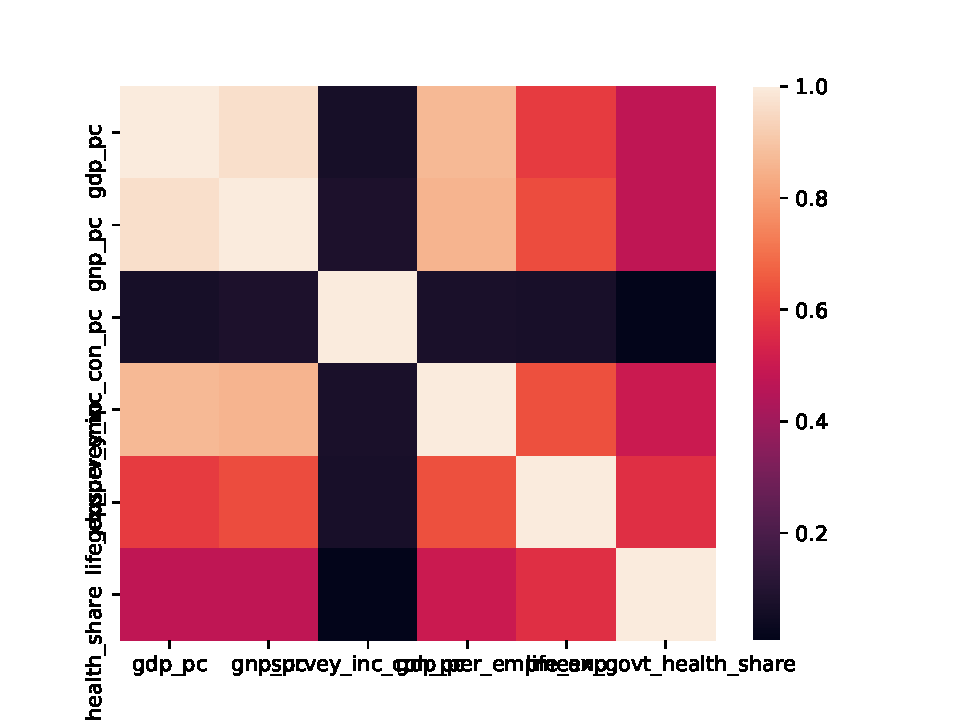
\includegraphics[width=\linewidth,keepaspectratio=true]{../Output/Figures/LE_Health_Econ_Correlations.pdf}
        \end{figure}

        \begin{figure}[h!]
            \centering
            \caption{Economic Measures PCA Loadings}
            \label{Econ_Loadings}	
            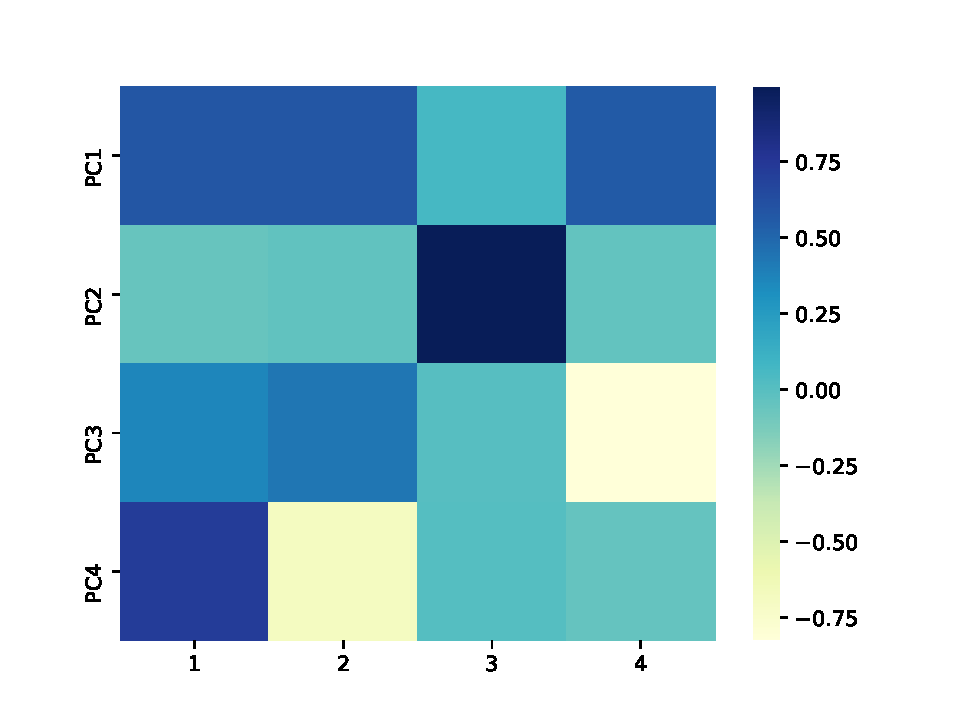
\includegraphics[width=\linewidth,keepaspectratio=true]{../Output/Figures/Econ_Indicator_Loadings.pdf}
        \end{figure}

        \begin{figure}[h!]
            \centering
            \caption{Economic Measures PCA Share of Variance Explained}
            \label{Econ_Share_Explained}	
            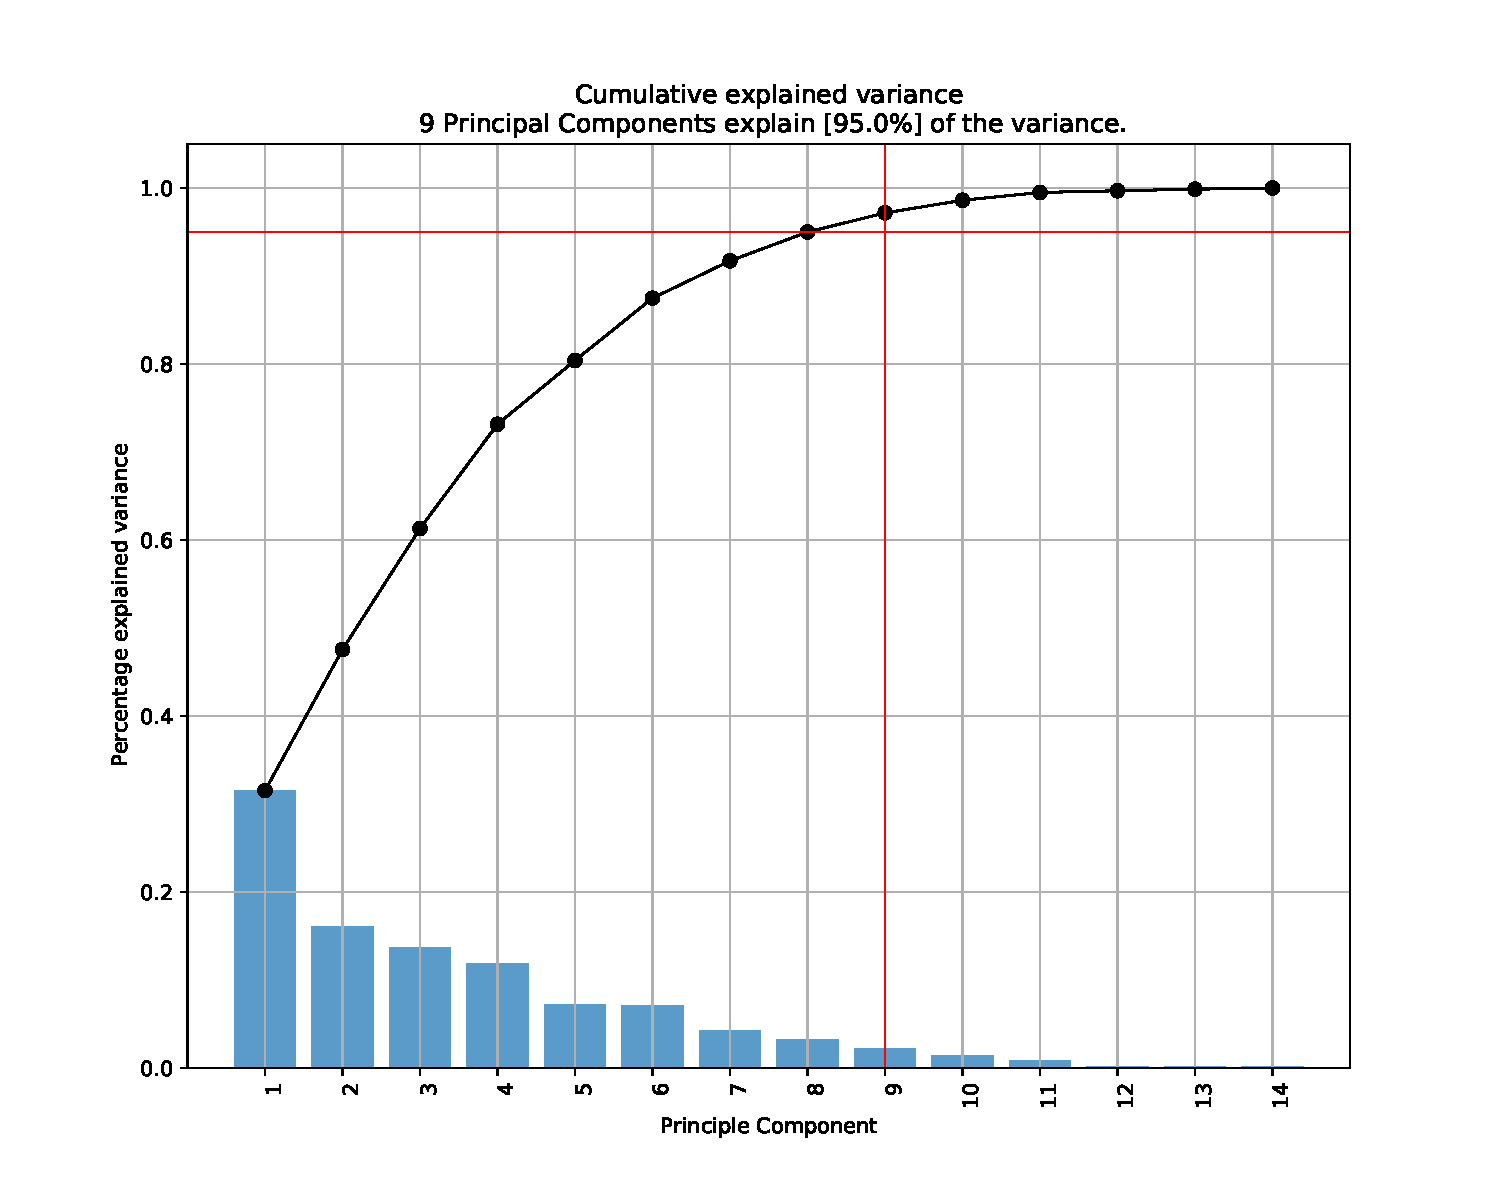
\includegraphics[width=\linewidth,keepaspectratio=true]{../Output/Figures/Econ_Indicator_Share_Explained.pdf}
        \end{figure}

\end{document}